\section{Conclusions}
\label{sec:conclusions}

The mathematical model of SEIQRS \cite{MingLiu,OldMingLiu} with a Small-World approximation for describing outbreak evolutions is here implemented and studied. Results present in literature are here validated and cross-checked.\\

The model is used to describe the COVID-19 virus spreading in Lombardy, Italy. Since March 1st, Lombardy's population is heavily hit by the spreading of this virus, causing thousends of deaths, and tens of thousands of hospitalised people. The Italian government has deployed strong laws to limit the sociality and contain the contagion. The model presented above is tuned and modified to better fit the Lombardy scenario, and describe better the collected data about the COVID-19 outbreak in the region.\\

A Profile Likelihood Fit is used to measure the model parameters against the collected data. This provides measurements for all the parameter, with associated uncertainties and correlations. The fit results for the parameters are used to generate a set of pseudo-experiments and estimate some features of the outbreak evolutions. The obtained  predictions  are compatible with data collected in Lombardy so far. Moreover the model predicts a saturation of the total cases of COVID-19 in Lombardy within a week around April 20th.\\


\begin{figure}
\centering
\subfloat {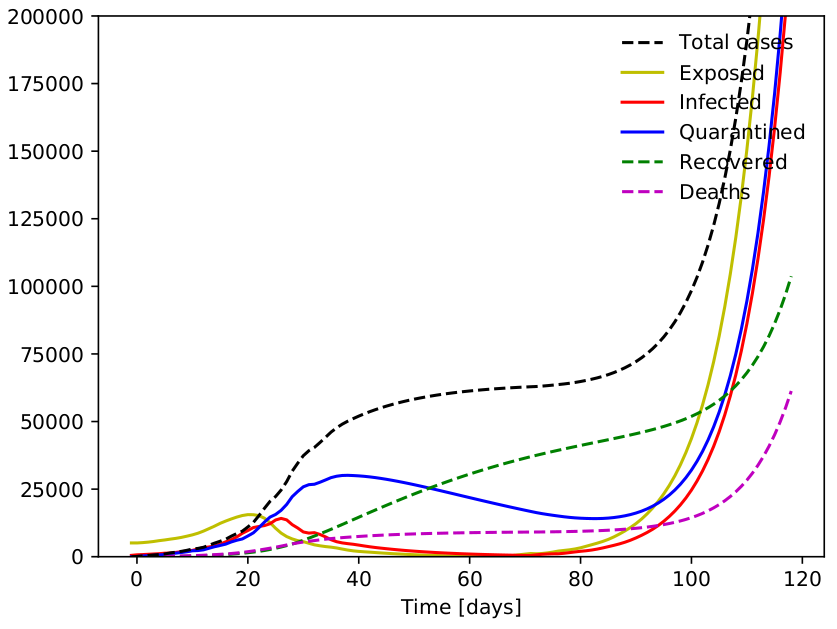
\includegraphics[width=0.4\textwidth]{imgs/Conclusions/Summary_reopening673.png}  }
\subfloat {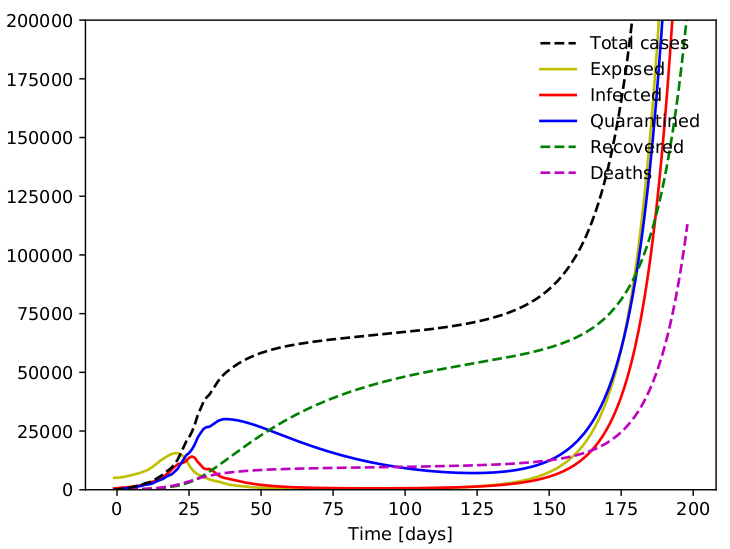
\includegraphics[width=0.4\textwidth]{imgs/Conclusions/Summary_reopening6months.png}  }
  \caption{Two exit strategies are here simulated: immediate reopening of all the activities on May 3rd (a) and gradual reopening over six months time (b).}
  \label{fig:reopening}
\end{figure}

The Italian government strategy is to prolongue the lock-down measures until May 3rd \cite{DPCM-1004}. The model used for the estimations above is used to estimate the effect of finishing the lock-down on that date. This is done by resetting the $\braket{k}$ parameter to the initial value on May 3rd in the model. The prediction is shown in Figure~\ref{fig:reopening}a. The prediction for a gradual reopening over six months is instead shown in Figure~\ref{fig:reopening}b. Since the levels of exposed and infected people do not go below the threshold for the outbreak (see Section~\ref{ssec:literature}), the outbreak occur again when the social interactions are restored to the nominal values. Therefore, without a vaccination campaign that could stop the contagion, the model indicates that the pre-outbreak level of interaction can be hardly restored even in a longer time.